%! alt Square ABCD with side 20, and the line MN through the midpoint M of BC and the point N on CD. The favourable region is shaded. On A's side of MN it is the pentagon M, Q, R, S, N, and on C's side it is the triangle M, N, P. The rays from A through Q and S are dashed.
%! after_paragraph 5
%! scale 7/20
% The shared preamble of every Kyuclid figure. pipeline/figures turns these colours into theme-aware paint,
% and refuses any other colour, so draw only with them:
%   figink (lines and labels), figaux (construction lines), figaccent (the object the argument turns on),
%   figtint and figaccenttint (light fills).
\documentclass[border=1.5pt]{standalone}
\usepackage{tkz-euclide}
\definecolor{figink}{RGB}{0,0,0}
\definecolor{figaux}{RGB}{85,85,85}
\definecolor{figaccent}{RGB}{192,57,43}
\definecolor{figtint}{RGB}{221,221,221}
\definecolor{figaccenttint}{RGB}{245,213,208}
% tkz-euclide's defaults draw circles, compasses and marks in 50% grey and fill points with a tint.
\makeatletter
\def\tkz@otherlinecolor{figink}
\def\tkz@euc@circlecolor{figink}
\def\tkz@euc@compasscolor{figink}
\def\tkz@euc@mkcolor{figink}
\def\tkz@mk@fill{figink}
\def\tkz@euc@pointfillcolor{figink}
\makeatother
\tkzSetUpLine[color=figink,line width=.7pt]
\tkzSetUpArc[color=figink,line width=.7pt]
\tkzSetUpCompass[color=figink,line width=.5pt]
\tkzSetUpPoint[color=figink,fill=figink,size=3.1pt]
\tikzset{
  every picture/.style={line cap=round,line join=round,color=figink},
  circle style/.append style={color=figink,line width=.7pt},
  aux/.style={color=figaux,line width=.45pt,dash pattern=on 2.6pt off 2pt},
  key/.style={color=figaccent,line width=1pt},
  mk/.style={color=figink,line width=.5pt},
  lbl/.style={color=figink,inner sep=2.2pt},
  len/.style={color=figink,inner sep=1.5pt,font=\small},
}

\begin{document}
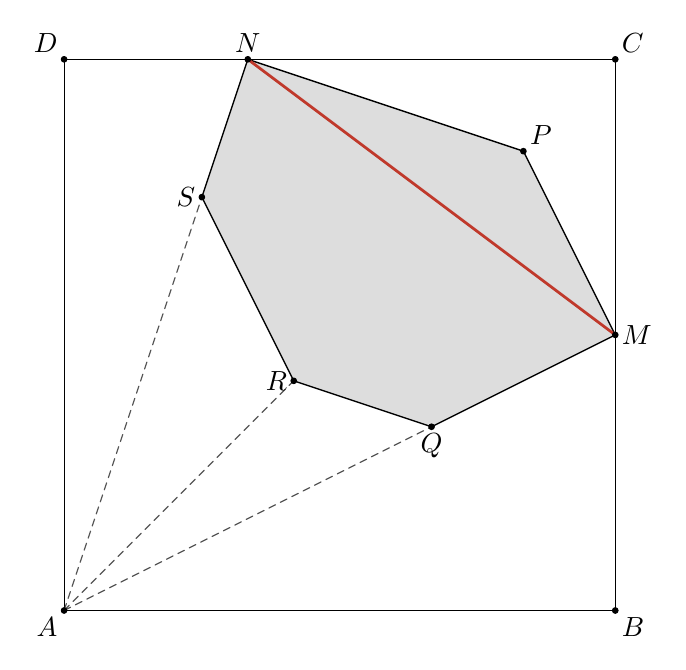
\begin{tikzpicture}
\tkzDefPoint(0.0,0.0){A} %! A = (0, 0)
\tkzDefPoint(7.0000000,0.0){B} %! B = (20, 0)
\tkzDefPoint(7.0000000,7.0000000){C} %! C = (20, 20)
\tkzDefPoint(0.0,7.0000000){D} %! D = (0, 20)
\tkzDefPoint(7.0000000,3.5000000){M} %! M = (20, 10)
\tkzDefPoint(2.3333333,7.0000000){N} %! N = (20/3, 20)
\tkzDefPoint(4.6666667,2.3333333){Q} %! Q = (40/3, 20/3)
\tkzDefPoint(2.9166667,2.9166667){R} %! R = (25/3, 25/3)
\tkzDefPoint(1.7500000,5.2500000){S} %! S = (5, 15)
\tkzDefPoint(5.8333333,5.8333333){P} %! P = (50/3, 50/3)
%! fact midpoint(M, B, C)
%! fact equal(dist(N, C), 2*dist(D, N))
%! fact collinear(A, Q, M)
%! fact collinear(A, S, N)
%! fact collinear(A, R, P)
%! fact dist(M, N) == 50/3
%! fact area(M, Q, R, S, N) == 875/9
%! fact area(M, N, P) == 250/9
%! fact equal(abs(3*x(R) + 4*y(R) - 100)/5, x(R))
%! fact equal(abs(3*x(R) + 4*y(R) - 100)/5, y(R))
%! fact equal(abs(3*x(P) + 4*y(P) - 100)/5, 20 - x(P))
%! fact equal(abs(3*x(P) + 4*y(P) - 100)/5, 20 - y(P))
\tkzFillPolygon[color=figtint](M,Q,R,S,N)
\tkzFillPolygon[color=figtint](M,N,P)
\tkzDrawPolygon(A,B,C,D)
\tkzDrawSegments[aux](A,Q A,S A,R)
\tkzDrawPolygon[line width=.5pt](M,Q,R,S,N)
\tkzDrawSegments[line width=.5pt](M,P N,P)
\tkzDrawSegment[key](M,N)
\tkzDrawPoints(A,B,C,D,M,N,Q,R,S,P)
\tkzLabelPoint[below left,lbl](A){$A$}
\tkzLabelPoint[below right,lbl](B){$B$}
\tkzLabelPoint[above right,lbl](C){$C$}
\tkzLabelPoint[above left,lbl](D){$D$}
\tkzLabelPoint[right,lbl](M){$M$}
\tkzLabelPoint[above,lbl](N){$N$}
\tkzLabelPoint[below,lbl](Q){$Q$}
\tkzLabelPoint[left,lbl](R){$R$}
\tkzLabelPoint[left,lbl](S){$S$}
\tkzLabelPoint[above right,lbl](P){$P$}
\end{tikzpicture}
\end{document}
